\documentclass{standalone}
\usepackage{tikz}
\usetikzlibrary{patterns, positioning}
\usepackage[sfdefault]{ClearSans} %% option 'sfdefault' activates Clear Sans as the default text font
\usepackage[T1]{fontenc}

\begin{document}
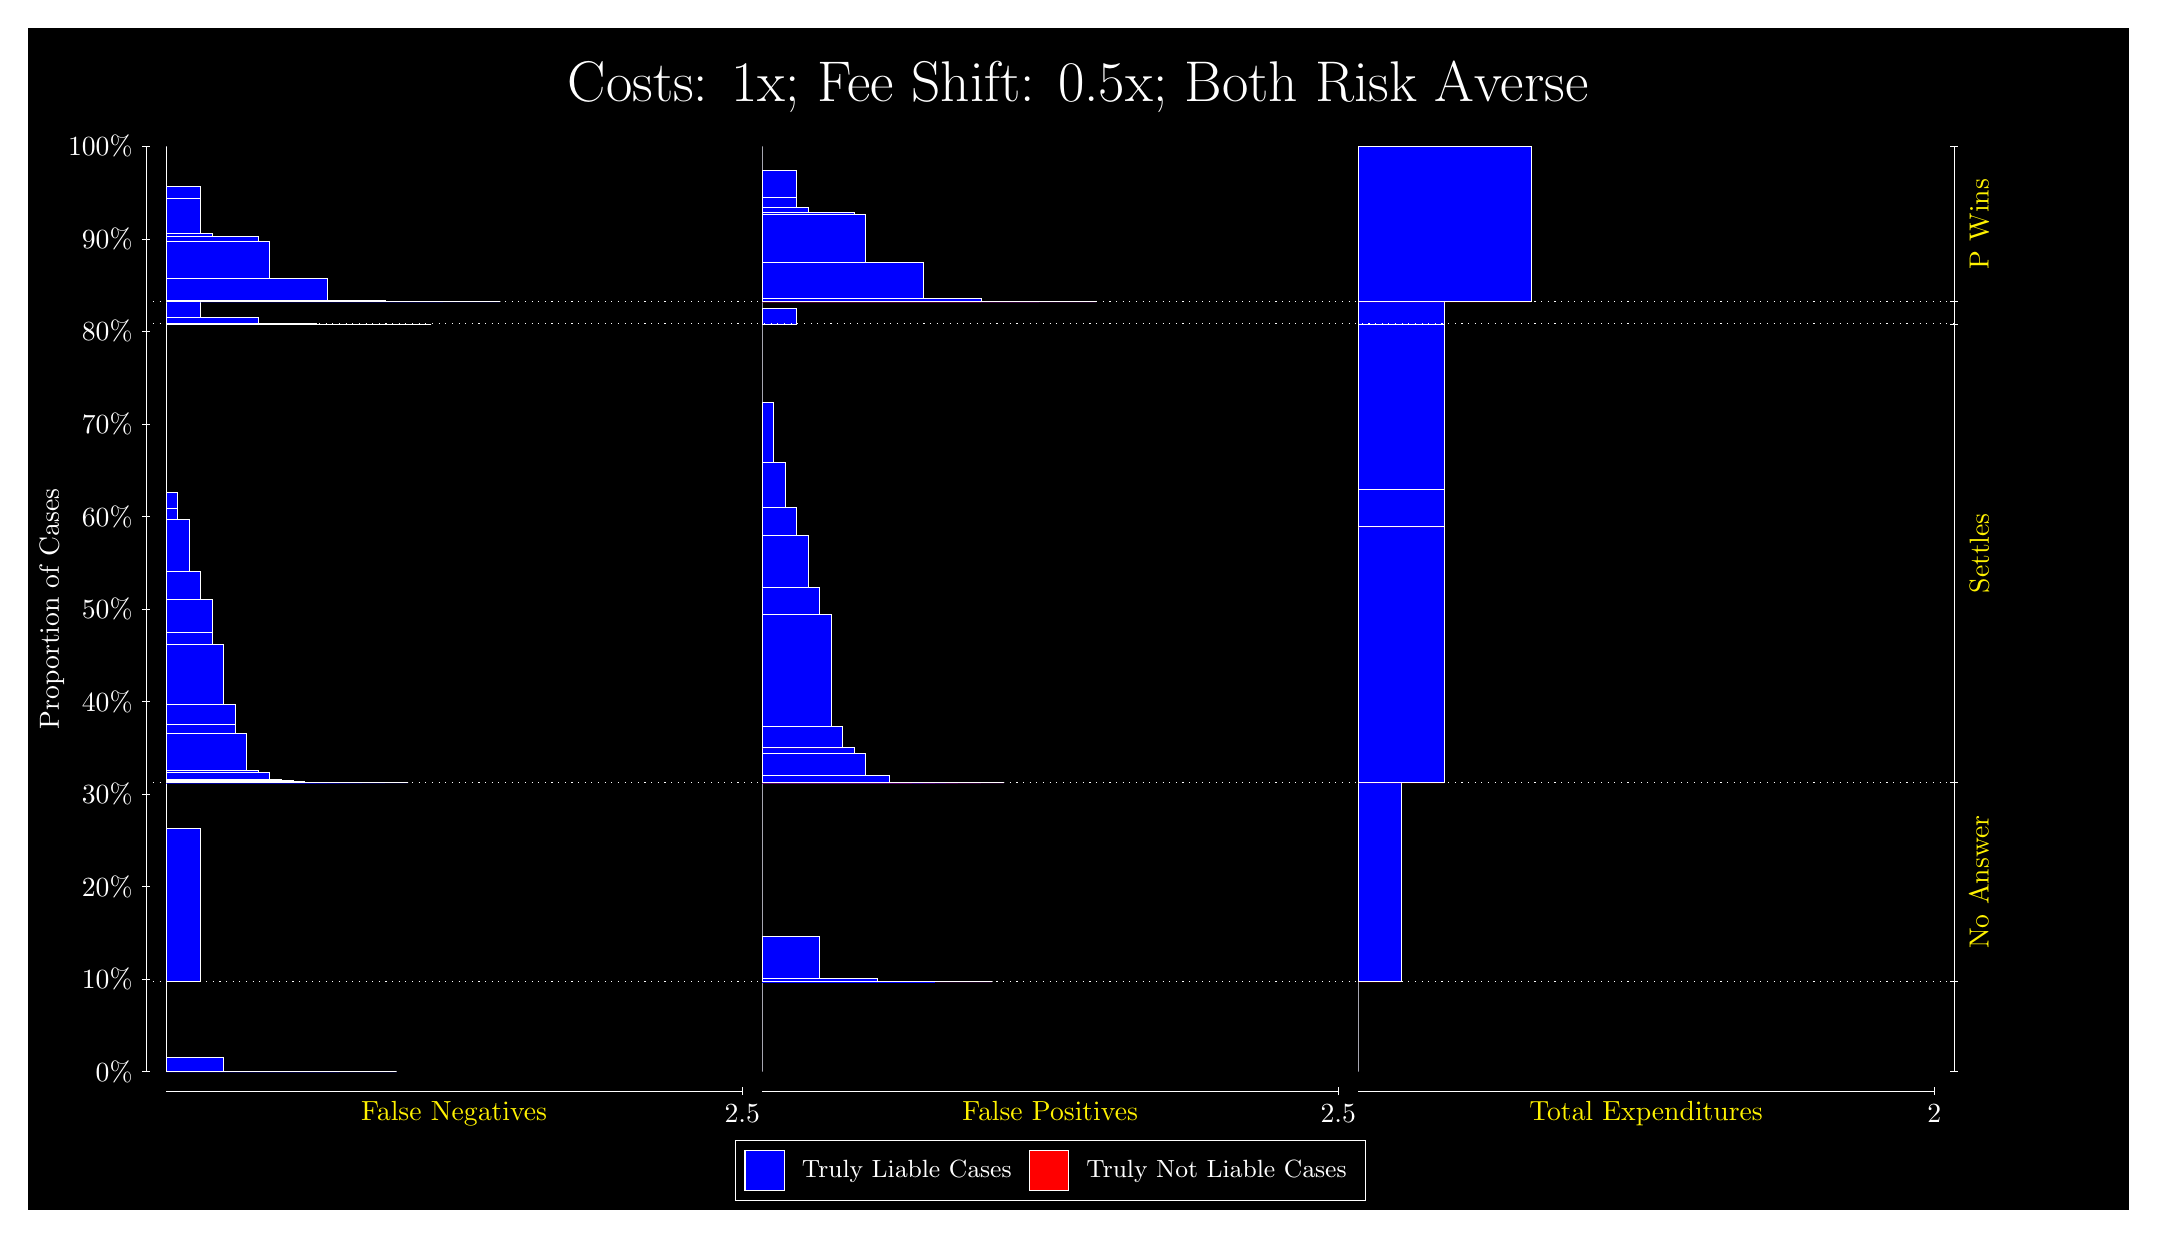
\begin{tikzpicture}
\draw[fill=black] (0,0) rectangle (26.667,15);
\draw[text=white] (0,13.5) rectangle (26.667,15) node[midway] {\huge Costs: 1x; Fee Shift: 0.5x; Both Risk Averse};
\draw[white, very thin] (1.5,1.75) -- (1.5,13.5);
\node[rotate=90, text=white, anchor=center] at (0.3, 7.625) {Proportion of Cases};
\draw[white, very thin] (1.45,1.75) -- (1.55,1.75);
\node[text=white, anchor=east] at (1.45, 1.75) {0\%};
\draw[white, very thin] (1.45,2.925) -- (1.55,2.925);
\node[text=white, anchor=east] at (1.45, 2.925) {10\%};
\draw[white, very thin] (1.45,4.1) -- (1.55,4.1);
\node[text=white, anchor=east] at (1.45, 4.1) {20\%};
\draw[white, very thin] (1.45,5.275) -- (1.55,5.275);
\node[text=white, anchor=east] at (1.45, 5.275) {30\%};
\draw[white, very thin] (1.45,6.45) -- (1.55,6.45);
\node[text=white, anchor=east] at (1.45, 6.45) {40\%};
\draw[white, very thin] (1.45,7.625) -- (1.55,7.625);
\node[text=white, anchor=east] at (1.45, 7.625) {50\%};
\draw[white, very thin] (1.45,8.8) -- (1.55,8.8);
\node[text=white, anchor=east] at (1.45, 8.8) {60\%};
\draw[white, very thin] (1.45,9.975) -- (1.55,9.975);
\node[text=white, anchor=east] at (1.45, 9.975) {70\%};
\draw[white, very thin] (1.45,11.15) -- (1.55,11.15);
\node[text=white, anchor=east] at (1.45, 11.15) {80\%};
\draw[white, very thin] (1.45,12.325) -- (1.55,12.325);
\node[text=white, anchor=east] at (1.45, 12.325) {90\%};
\draw[white, very thin] (1.45,13.5) -- (1.55,13.5);
\node[text=white, anchor=east] at (1.45, 13.5) {100\%};

\draw[white, very thin] (24.457,1.75) -- (24.457,13.5);
\draw[white, very thin] (24.407,1.75) -- (24.507,1.75);
\node[anchor=west] at (24.407, 1.75) {};
\draw[white, very thin] (24.407,2.8901) -- (24.507,2.8901);
\node[anchor=west] at (24.407, 2.8901) {};
\draw[white, very thin] (24.407,5.4202) -- (24.507,5.4202);
\node[anchor=west] at (24.407, 5.4202) {};
\draw[white, very thin] (24.407,11.246) -- (24.507,11.246);
\node[anchor=west] at (24.407, 11.246) {};
\draw[white, very thin] (24.407,11.527) -- (24.507,11.527);
\node[anchor=west] at (24.407, 11.527) {};
\draw[white, very thin] (24.407,13.5) -- (24.507,13.5);
\node[anchor=west] at (24.407, 13.5) {};

\draw[white, very thin, fill=blue] (1.75,1.75) rectangle (4.6775,1.75);
\draw[white, very thin, fill=blue] (1.75,1.75) rectangle (3.9457,1.75);
\draw[white, very thin, fill=blue] (1.75,1.75) rectangle (3.2138,1.7516);
\draw[white, very thin, fill=blue] (1.75,1.7516) rectangle (2.4819,1.9367);
\draw[white, very thin, fill=red] (1.75,1.9367) rectangle (1.75,1.9367);
\draw[white, very thin, fill=blue] (1.75,1.9367) rectangle (1.75,2.8901);
\draw[white, very thin, fill=blue] (1.75,2.8901) rectangle (2.1891,4.8423);
\draw[white, very thin, fill=red] (1.75,4.8423) rectangle (1.75,4.8423);
\draw[white, very thin, fill=blue] (1.75,4.8423) rectangle (1.75,5.4202);
\draw[white, very thin, fill=blue] (1.75,5.4202) rectangle (4.8239,5.4202);
\draw[white, very thin, fill=blue] (1.75,5.4202) rectangle (4.5312,5.4202);
\draw[white, very thin, fill=blue] (1.75,5.4202) rectangle (4.2384,5.4202);
\draw[white, very thin, fill=blue] (1.75,5.4202) rectangle (4.092,5.4202);
\draw[white, very thin, fill=blue] (1.75,5.4202) rectangle (3.9457,5.4202);
\draw[white, very thin, fill=blue] (1.75,5.4202) rectangle (3.7993,5.4203);
\draw[white, very thin, fill=blue] (1.75,5.4203) rectangle (3.6529,5.4204);
\draw[white, very thin, fill=blue] (1.75,5.4204) rectangle (3.5065,5.4353);
\draw[white, very thin, fill=blue] (1.75,5.4353) rectangle (3.3602,5.4446);
\draw[white, very thin, fill=blue] (1.75,5.4446) rectangle (3.2138,5.4593);
\draw[white, very thin, fill=blue] (1.75,5.4593) rectangle (3.0674,5.4623);
\draw[white, very thin, fill=blue] (1.75,5.4623) rectangle (3.0674,5.5507);
\draw[white, very thin, fill=blue] (1.75,5.5507) rectangle (2.921,5.5712);
\draw[white, very thin, fill=blue] (1.75,5.5712) rectangle (2.7746,6.0442);
\draw[white, very thin, fill=blue] (1.75,6.0442) rectangle (2.6283,6.1584);
\draw[white, very thin, fill=blue] (1.75,6.1584) rectangle (2.6283,6.4184);
\draw[white, very thin, fill=blue] (1.75,6.4184) rectangle (2.4819,7.1755);
\draw[white, very thin, fill=blue] (1.75,7.1755) rectangle (2.3355,7.3255);
\draw[white, very thin, fill=blue] (1.75,7.3255) rectangle (2.3355,7.7526);
\draw[white, very thin, fill=blue] (1.75,7.7526) rectangle (2.1891,8.1027);
\draw[white, very thin, fill=blue] (1.75,8.1027) rectangle (2.0428,8.7697);
\draw[white, very thin, fill=blue] (1.75,8.7697) rectangle (2.0428,8.7697);
\draw[white, very thin, fill=blue] (1.75,8.7697) rectangle (1.8964,8.9032);
\draw[white, very thin, fill=blue] (1.75,8.9032) rectangle (1.8964,9.1064);
\draw[white, very thin, fill=red] (1.75,9.1064) rectangle (1.75,9.1064);
\draw[white, very thin, fill=blue] (1.75,9.1064) rectangle (1.75,11.246);
\draw[white, very thin, fill=blue] (1.75,11.246) rectangle (5.1167,11.246);
\draw[white, very thin, fill=blue] (1.75,11.246) rectangle (4.3848,11.246);
\draw[white, very thin, fill=blue] (1.75,11.246) rectangle (3.6529,11.253);
\draw[white, very thin, fill=blue] (1.75,11.253) rectangle (2.921,11.327);
\draw[white, very thin, fill=blue] (1.75,11.327) rectangle (2.1891,11.527);
\draw[white, very thin, fill=red] (1.75,11.527) rectangle (1.75,11.527);
\draw[white, very thin, fill=blue] (1.75,11.527) rectangle (5.9949,11.527);
\draw[white, very thin, fill=blue] (1.75,11.527) rectangle (5.2631,11.527);
\draw[white, very thin, fill=blue] (1.75,11.527) rectangle (4.5312,11.55);
\draw[white, very thin, fill=blue] (1.75,11.55) rectangle (4.3848,11.55);
\draw[white, very thin, fill=blue] (1.75,11.55) rectangle (3.7993,11.827);
\draw[white, very thin, fill=blue] (1.75,11.827) rectangle (3.6529,11.827);
\draw[white, very thin, fill=blue] (1.75,11.827) rectangle (3.0674,12.296);
\draw[white, very thin, fill=blue] (1.75,12.296) rectangle (2.921,12.358);
\draw[white, very thin, fill=blue] (1.75,12.358) rectangle (2.3355,12.39);
\draw[white, very thin, fill=blue] (1.75,12.39) rectangle (2.1891,12.841);
\draw[white, very thin, fill=blue] (1.75,12.841) rectangle (2.1891,12.994);
\draw[white, very thin, fill=red] (1.75,12.994) rectangle (1.75,12.994);
\draw[white, very thin, fill=blue] (1.75,12.994) rectangle (1.75,13.5);
\draw[white, very thin, fill=red] (9.3189,1.75) rectangle (9.3189,1.75);
\draw[white, very thin, fill=blue] (9.3189,1.75) rectangle (9.3189,2.8901);
\draw[white, very thin, fill=red] (9.3189,2.8901) rectangle (12.246,2.8901);
\draw[white, very thin, fill=blue] (9.3189,2.8901) rectangle (12.246,2.8901);
\draw[white, very thin, fill=blue] (9.3189,2.8901) rectangle (11.515,2.8904);
\draw[white, very thin, fill=blue] (9.3189,2.8904) rectangle (10.783,2.9318);
\draw[white, very thin, fill=blue] (9.3189,2.9318) rectangle (10.051,3.468);
\draw[white, very thin, fill=blue] (9.3189,3.468) rectangle (9.3189,5.4202);
\draw[white, very thin, fill=red] (9.3189,5.4202) rectangle (12.393,5.4202);
\draw[white, very thin, fill=blue] (9.3189,5.4202) rectangle (12.393,5.4202);
\draw[white, very thin, fill=red] (9.3189,5.4202) rectangle (12.1,5.4202);
\draw[white, very thin, fill=blue] (9.3189,5.4202) rectangle (12.1,5.4202);
\draw[white, very thin, fill=red] (9.3189,5.4202) rectangle (11.807,5.4202);
\draw[white, very thin, fill=blue] (9.3189,5.4202) rectangle (11.807,5.4202);
\draw[white, very thin, fill=blue] (9.3189,5.4202) rectangle (11.661,5.4202);
\draw[white, very thin, fill=red] (9.3189,5.4202) rectangle (11.515,5.4202);
\draw[white, very thin, fill=blue] (9.3189,5.4202) rectangle (11.515,5.4202);
\draw[white, very thin, fill=blue] (9.3189,5.4202) rectangle (11.368,5.4203);
\draw[white, very thin, fill=red] (9.3189,5.4203) rectangle (11.222,5.4203);
\draw[white, very thin, fill=blue] (9.3189,5.4203) rectangle (11.222,5.428);
\draw[white, very thin, fill=blue] (9.3189,5.428) rectangle (11.075,5.4283);
\draw[white, very thin, fill=red] (9.3189,5.4283) rectangle (10.929,5.4283);
\draw[white, very thin, fill=blue] (9.3189,5.4283) rectangle (10.929,5.5138);
\draw[white, very thin, fill=blue] (9.3189,5.5138) rectangle (10.783,5.5149);
\draw[white, very thin, fill=blue] (9.3189,5.5149) rectangle (10.636,5.5151);
\draw[white, very thin, fill=red] (9.3189,5.5151) rectangle (10.636,5.5151);
\draw[white, very thin, fill=blue] (9.3189,5.5151) rectangle (10.636,5.7919);
\draw[white, very thin, fill=blue] (9.3189,5.7919) rectangle (10.49,5.8632);
\draw[white, very thin, fill=red] (9.3189,5.8632) rectangle (10.344,5.8632);
\draw[white, very thin, fill=blue] (9.3189,5.8632) rectangle (10.344,6.1349);
\draw[white, very thin, fill=blue] (9.3189,6.1349) rectangle (10.197,7.5597);
\draw[white, very thin, fill=red] (9.3189,7.5597) rectangle (10.051,7.5597);
\draw[white, very thin, fill=blue] (9.3189,7.5597) rectangle (10.051,7.8963);
\draw[white, very thin, fill=blue] (9.3189,7.8963) rectangle (9.9044,7.8963);
\draw[white, very thin, fill=blue] (9.3189,7.8963) rectangle (9.9044,8.5633);
\draw[white, very thin, fill=blue] (9.3189,8.5633) rectangle (9.758,8.9134);
\draw[white, very thin, fill=blue] (9.3189,8.9134) rectangle (9.6116,9.4906);
\draw[white, very thin, fill=blue] (9.3189,9.4906) rectangle (9.4652,10.248);
\draw[white, very thin, fill=blue] (9.3189,10.248) rectangle (9.3189,11.246);
\draw[white, very thin, fill=red] (9.3189,11.246) rectangle (9.758,11.246);
\draw[white, very thin, fill=blue] (9.3189,11.246) rectangle (9.758,11.445);
\draw[white, very thin, fill=blue] (9.3189,11.445) rectangle (9.3189,11.527);
\draw[white, very thin, fill=red] (9.3189,11.527) rectangle (13.564,11.527);
\draw[white, very thin, fill=blue] (9.3189,11.527) rectangle (13.564,11.527);
\draw[white, very thin, fill=red] (9.3189,11.527) rectangle (12.832,11.527);
\draw[white, very thin, fill=blue] (9.3189,11.527) rectangle (12.832,11.527);
\draw[white, very thin, fill=red] (9.3189,11.527) rectangle (12.1,11.527);
\draw[white, very thin, fill=blue] (9.3189,11.527) rectangle (12.1,11.568);
\draw[white, very thin, fill=red] (9.3189,11.568) rectangle (11.368,11.568);
\draw[white, very thin, fill=blue] (9.3189,11.568) rectangle (11.368,12.033);
\draw[white, very thin, fill=red] (9.3189,12.033) rectangle (11.222,12.033);
\draw[white, very thin, fill=blue] (9.3189,12.033) rectangle (11.222,12.033);
\draw[white, very thin, fill=blue] (9.3189,12.033) rectangle (10.636,12.637);
\draw[white, very thin, fill=red] (9.3189,12.637) rectangle (10.49,12.637);
\draw[white, very thin, fill=blue] (9.3189,12.637) rectangle (10.49,12.668);
\draw[white, very thin, fill=blue] (9.3189,12.668) rectangle (9.9044,12.73);
\draw[white, very thin, fill=blue] (9.3189,12.73) rectangle (9.758,12.856);
\draw[white, very thin, fill=red] (9.3189,12.856) rectangle (9.758,12.856);
\draw[white, very thin, fill=blue] (9.3189,12.856) rectangle (9.758,13.2);
\draw[white, very thin, fill=blue] (9.3189,13.2) rectangle (9.3189,13.5);
\draw[white, very thin, fill=red] (16.888,1.75) rectangle (16.888,1.75);
\draw[white, very thin, fill=blue] (16.888,1.75) rectangle (16.888,2.8901);
\draw[white, very thin, fill=red] (16.888,2.8901) rectangle (17.437,2.8901);
\draw[white, very thin, fill=blue] (16.888,2.8901) rectangle (17.437,5.4202);
\draw[white, very thin, fill=red] (16.888,5.4202) rectangle (17.986,5.4202);
\draw[white, very thin, fill=blue] (16.888,5.4202) rectangle (17.986,8.6712);
\draw[white, very thin, fill=red] (16.888,8.6712) rectangle (17.986,8.6712);
\draw[white, very thin, fill=blue] (16.888,8.6712) rectangle (17.986,9.1433);
\draw[white, very thin, fill=red] (16.888,9.1433) rectangle (17.986,9.1433);
\draw[white, very thin, fill=blue] (16.888,9.1433) rectangle (17.986,11.246);
\draw[white, very thin, fill=red] (16.888,11.246) rectangle (17.986,11.246);
\draw[white, very thin, fill=blue] (16.888,11.246) rectangle (17.986,11.527);
\draw[white, very thin, fill=red] (16.888,11.527) rectangle (19.083,11.527);
\draw[white, very thin, fill=blue] (16.888,11.527) rectangle (19.083,13.5);
\draw[white, dotted] (1.5,2.8901) -- (24.457,2.8901);
\draw[white, dotted] (1.5,5.4202) -- (24.457,5.4202);
\draw[white, dotted] (1.5,11.246) -- (24.457,11.246);
\draw[white, dotted] (1.5,11.527) -- (24.457,11.527);
\draw[white, very thin] (1.75,1.5) -- (9.0689,1.5);
\node[text=yellow, anchor=north] at (5.4094, 1.5) {False Negatives};
\draw[white, very thin] (9.0689,1.45) -- (9.0689,1.55);
\node[text=white, anchor=north] at (9.0689, 1.45) {2.5};

\draw[white, very thin] (9.3189,1.5) -- (16.638,1.5);
\node[text=yellow, anchor=north] at (12.978, 1.5) {False Positives};
\draw[white, very thin] (16.638,1.45) -- (16.638,1.55);
\node[text=white, anchor=north] at (16.638, 1.45) {2.5};

\draw[white, very thin] (16.888,1.5) -- (24.207,1.5);
\node[text=yellow, anchor=north] at (20.547, 1.5) {Total Expenditures};
\draw[white, very thin] (24.207,1.45) -- (24.207,1.55);
\node[text=white, anchor=north] at (24.207, 1.45) {2};


\node[text=yellow, centered, rotate=90] at (24.777, 4.1552) {No Answer};
\node[text=yellow, centered, rotate=90] at (24.777, 8.333) {Settles};

\node[text=yellow, centered, rotate=90] at (24.777, 12.513) {P Wins};

\draw (12.978300999999998,1.5) node[draw=none] (baseCoordinate) {};
\begin{scope}[align=center]
        \matrix[scale=0.5, draw=white, below=0.5cm of baseCoordinate, nodes={draw}, column sep=0.1cm]{
            \node[rectangle, draw, minimum width=0.5cm, minimum height=0.5cm, fill=blue] {}; &
            \node[draw=none, font=\small, text=white] (B) {Truly Liable Cases}; &
            \node[rectangle, draw, minimum width=0.5cm, minimum height=0.5cm, fill=red] {}; &
            \node[draw=none, font=\small, text=white] (B) {Truly Not Liable Cases}; \\
            };
\end{scope}

\end{tikzpicture}
\end{document}